\section{Free planning search preserves strong reference behavior}
\label{sec:native-planning-search}
\subsection{A separate finite objective-conditioned study}
The preceding three-arm comparison establishes an operative planning path,
not what a search invents. We next permit original catalog assignment in a
separate count/content search. Five initial fixed Qwen3-8B university
researchers and other native actors run for four years against the same
103,107-record corpus. Base resources remain30, the project-output cap remains
two, and the annual funding fraction remains0.2. Native production, costs,
calendar and accounting are unchanged. Institutions may edit source, nodes,
protocols, wiring and schedules; catalog assignments must preserve the actual
displayed topic, content and duration. Existing projects cannot be shortened.
This named design scope is not the limit of the broader system framework.

The losses remain $T=-N$, where $N$ counts accepted decisions, and
$U=-\sum_{j\in\mathcal A}(\overline q_j-3)$, where the three-position
fixed-content panel supplies an abstract-based opinion. These opinions are
not scientific truth. P and resource histories are diagnostics, not additional
objectives or constraints. Eight fresh developer references share the permitted
authority (Table~\ref{tab:planning-all}). Three proposal slots per objective
use the installed local35B designer at optimizer seed68011. The interleaved
order is T0,U0,U1,T1,T2,U2. Each editing parent is selected by assigned loss
from the common references and own completed history; all14 worlds explicitly
reuse development seed61001. These are two histories, not independent optimizer
replications or unused-condition evaluations.

All six programs submit and complete. Final selection is the earliest tied
completed own submission, T0 or U0, with all three own ties retained per
objective. No reference fallback, novelty requirement, participation floor
or improvement veto is added. Two original-source audits and cost projections
agree; five pairs of score, choice, effect, complete-input and signed-content
exports agree. The stopped initial calibration remains separate from this
normally closed second attempt, with its unknown response costs retained.

\begin{table}[t]
\centering\small
\begin{tabular}{llrrc}
\toprule
ID & Institution or own submission & T & U & Point\\
\midrule
R1 & No agenda effect, reserve21, reviewed all & $-12$ & $-8$ & G5\\
R2 & Advisory agenda, reserve21, reviewed all & $-18$ & $-11.3333$ & G3\\
R3 & Assignment, reserve21, reviewed all & $-18$ & $-13$ & G2\\
R4 & Assignment, reserve10, reviewed all & $-12$ & $-8$ & G5\\
R5 & Assignment, equalization, reviewed all & $-12$ & $-8$ & G5\\
R6 & Assignment, reserve21, native threshold3 & $-18$ & $-13$ & G2\\
R7 & Assignment, reserve21, no-review all & $-18$ & $-13.3333$ & G1\\
R8 & Assignment, reserve21, no-review reject & $0$ & $0$ & G6\\
\midrule
T0 & First count proposal, selected & $-18$ & $-10.3333$ & G4\\
U0 & First content proposal, selected & $-18$ & $-13.3333$ & G1\\
U1 & Content redesign & $-18$ & $-13.3333$ & G1\\
T1 & Count redesign & $-18$ & $-11.3333$ & G3\\
T2 & Last count proposal & $-18$ & $-10.3333$ & G4\\
U2 & Last content proposal & $-18$ & $-13.3333$ & G1\\
\bottomrule
\end{tabular}
\caption{All eight fresh references and six own proposals, in execution order.
Every own assigned loss ties its best fresh reference. Display rounding does
not determine ties: selection and analysis retain original floating-point
losses. Point labels map every exact tie in Figure~\ref{fig:planning-cross}.}
\label{tab:planning-all}
\end{table}

\subsection{Content preferences refine observed count ties}
Every own count loss is$-18$ and every own content loss is approximately
$-13.3333$ (Figure~\ref{fig:planning-paths}). The selected U institution has
observed U lower by3 than selected T, at equal T. Parent selection belongs to
the declared objective-conditioned procedure: all T parents are R2, and all U
parents are R7. Their difference is a valid observation of the end-to-end
procedure, not an isolated gain caused by the generated edit or a general
expected objective-label effect from one history per branch.

\begin{figure}[t]
\centering
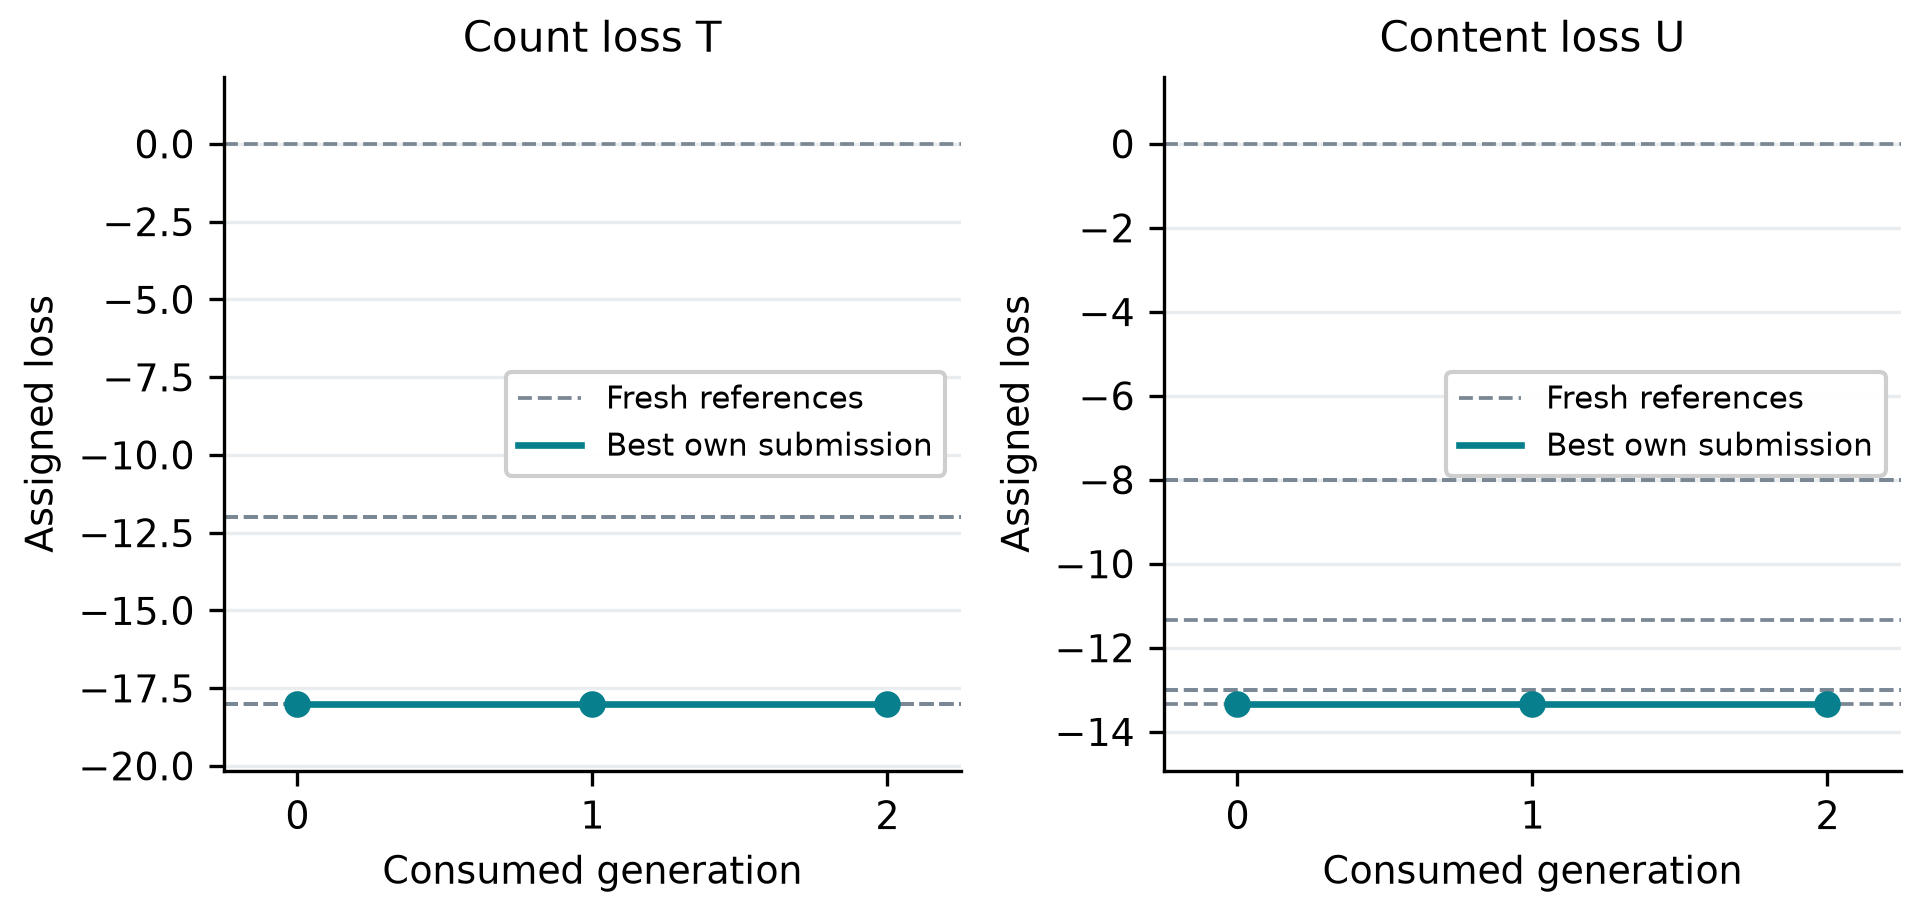
\includegraphics[width=\linewidth]{figures/native-planning-paper-v1/loss-paths.png}
\caption{All three consumed proposals per objective and the unchanged fresh
reference losses. Overlapping gray lines retain the eight references listed
in Table~\ref{tab:planning-all}. Own losses and incumbent paths are flat;
this is not independent-seed uncertainty or evidence of generated advantage.}
\label{fig:planning-paths}
\end{figure}

R7 minimizes U and is also one of four references minimizing T. The complete
14-world archive therefore has overlapping, but unequal, minimum sets.
Of91 pairs,43 have the same strict preference,36 tie only in T and12 tie in
both losses; none has a strict preference conflict. U refines part of a
count-neutral plateau rather than revealing an observed unavoidable trade-off
(Figure~\ref{fig:planning-cross}). This finite archive is not a global frontier
or an upper bound on attainable institutional performance.

\begin{figure}[t]
\centering
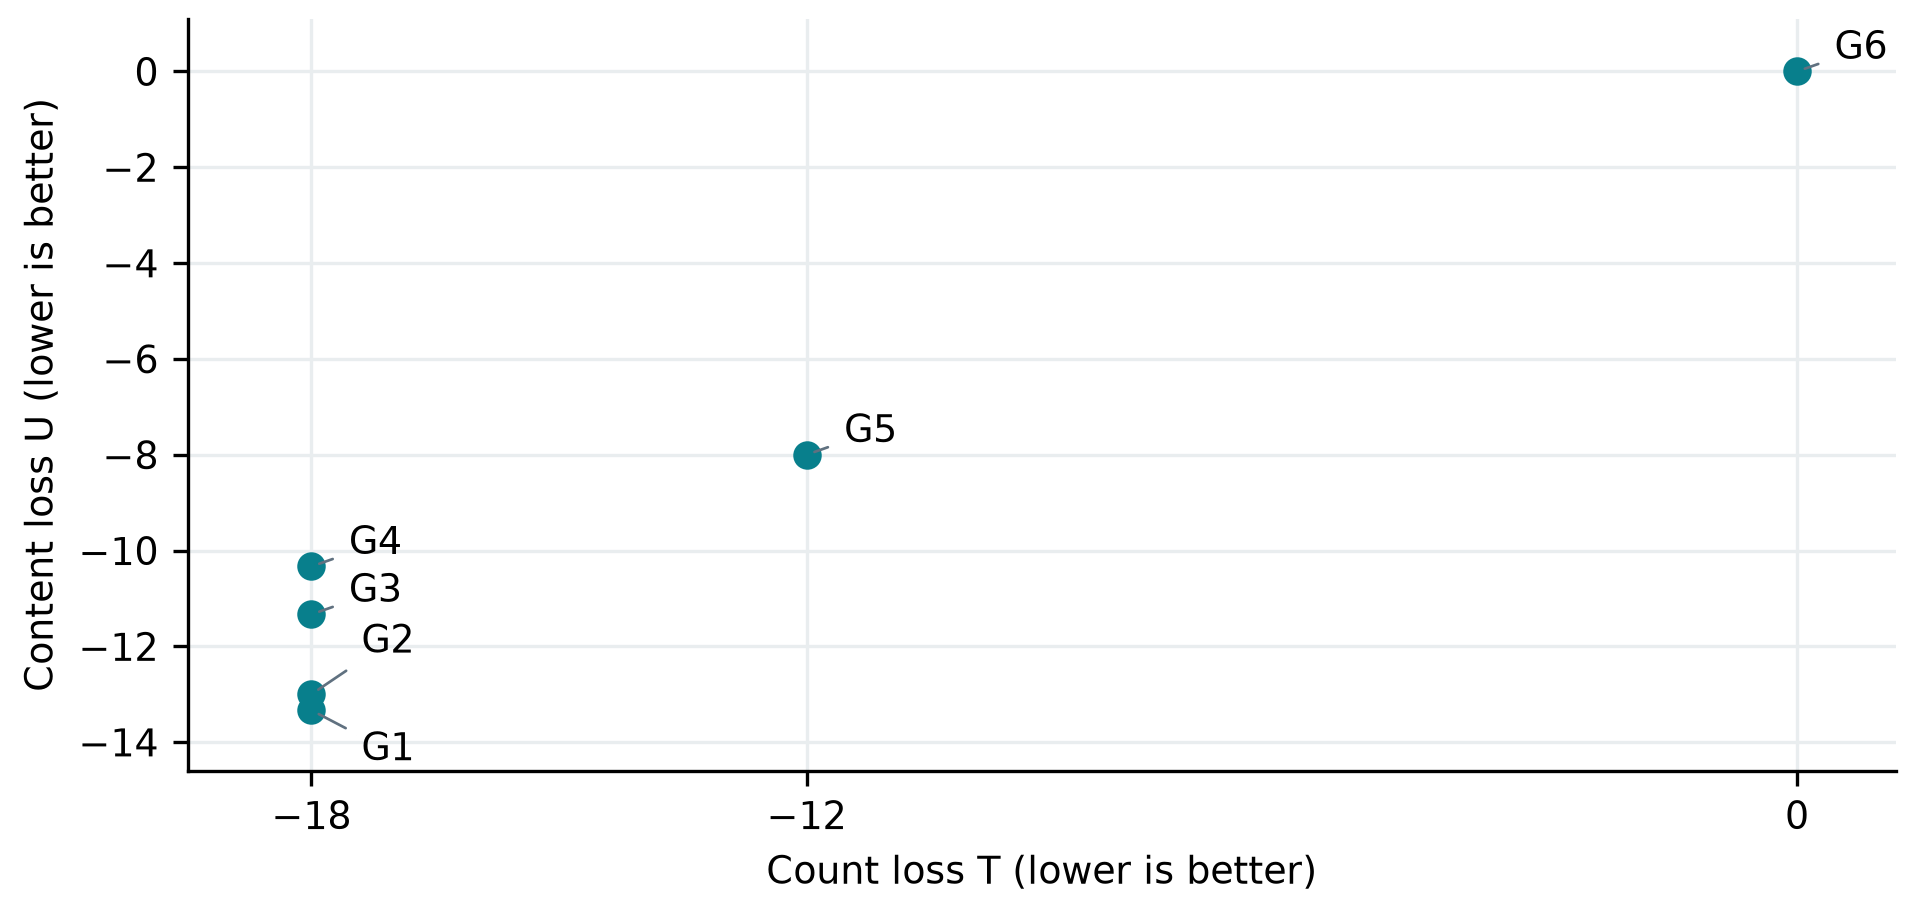
\includegraphics[width=\linewidth]{figures/native-planning-paper-v1/cross-scores.png}
\caption{Both losses on all14 completed native worlds, grouped only at exact
shared score coordinates. Table~\ref{tab:planning-all} retains every label.
Annotations move for legibility; data coordinates are not jittered. G1 belongs
to both observed minimum sets. Different selected institutions do not imply
that the objectives must trade off.}
\label{fig:planning-cross}
\end{figure}

\subsection{Literal code edits versus actual researcher behavior}
All six submitted programs change only \code{world.selection} source, explicitly
accepting all papers from parents already configured accept-all. No program
changes planning, allocation, nodes, wiring or schedules. T0 and T2 also set
\code{final\_score=1.0}; T1 retains mean native review scores. The U programs
retain mean scores, with a default-valued field lookup in U0. A literal source
change or equal assigned loss does not prove behavioral equivalence.

The complete-input reader instead finds eight exact observed-input classes.
U0/U1/U2 and R7 have identical ordered full scientist payloads and literal
response choices. T1 likewise matches R2. T0 and T2 match each other but differ
from R2, with outside U worse by1. Full provider envelopes differ within these
multi-world classes. Equality on these observed paths is not equivalence on
unobserved histories or permission to merge different policies in future runs.

Each T program retains ten original direction calls and no catalog assignment;
each U program retains ten validated assignments and no direction call.
All own annual active-founder paths are5,5,4,2. The effect trace retains336
code calls and56 committed annual boundaries across all14 worlds. Literal
first plans predominantly target selection and adjacent scoring code. U2
also proposes editing the catalog agenda, but its final program does not.
The plans include mistaken hypotheses about already all-accept parents.
This documents narrow actual exploration; it does not identify parent
presentation, file ordering, incentives or designer capability as its cause.

\subsection{Signed content support and measured cost}
The216 accepted occurrences represent54 unique contents. Every observed
centered contribution is positive or zero, never negative
(Figure~\ref{fig:planning-content}). R7 and each U proposal have13 positive
and5 zero occurrences; T0/T2 have10 positive and8 zero occurrences. Rational
utilities40/3 and31/3 explain those latter sums but never replace operational
floating-point losses. For a fixed accepted multiset, discarding a positive
contribution cannot increase total utility. A selective institution may still
change future production and the multiset; rejected or unproduced content is
not rerated. Occurrences, unique contents and critic errors are not independent
replicates of the same estimand.

\begin{figure}[t]
\centering
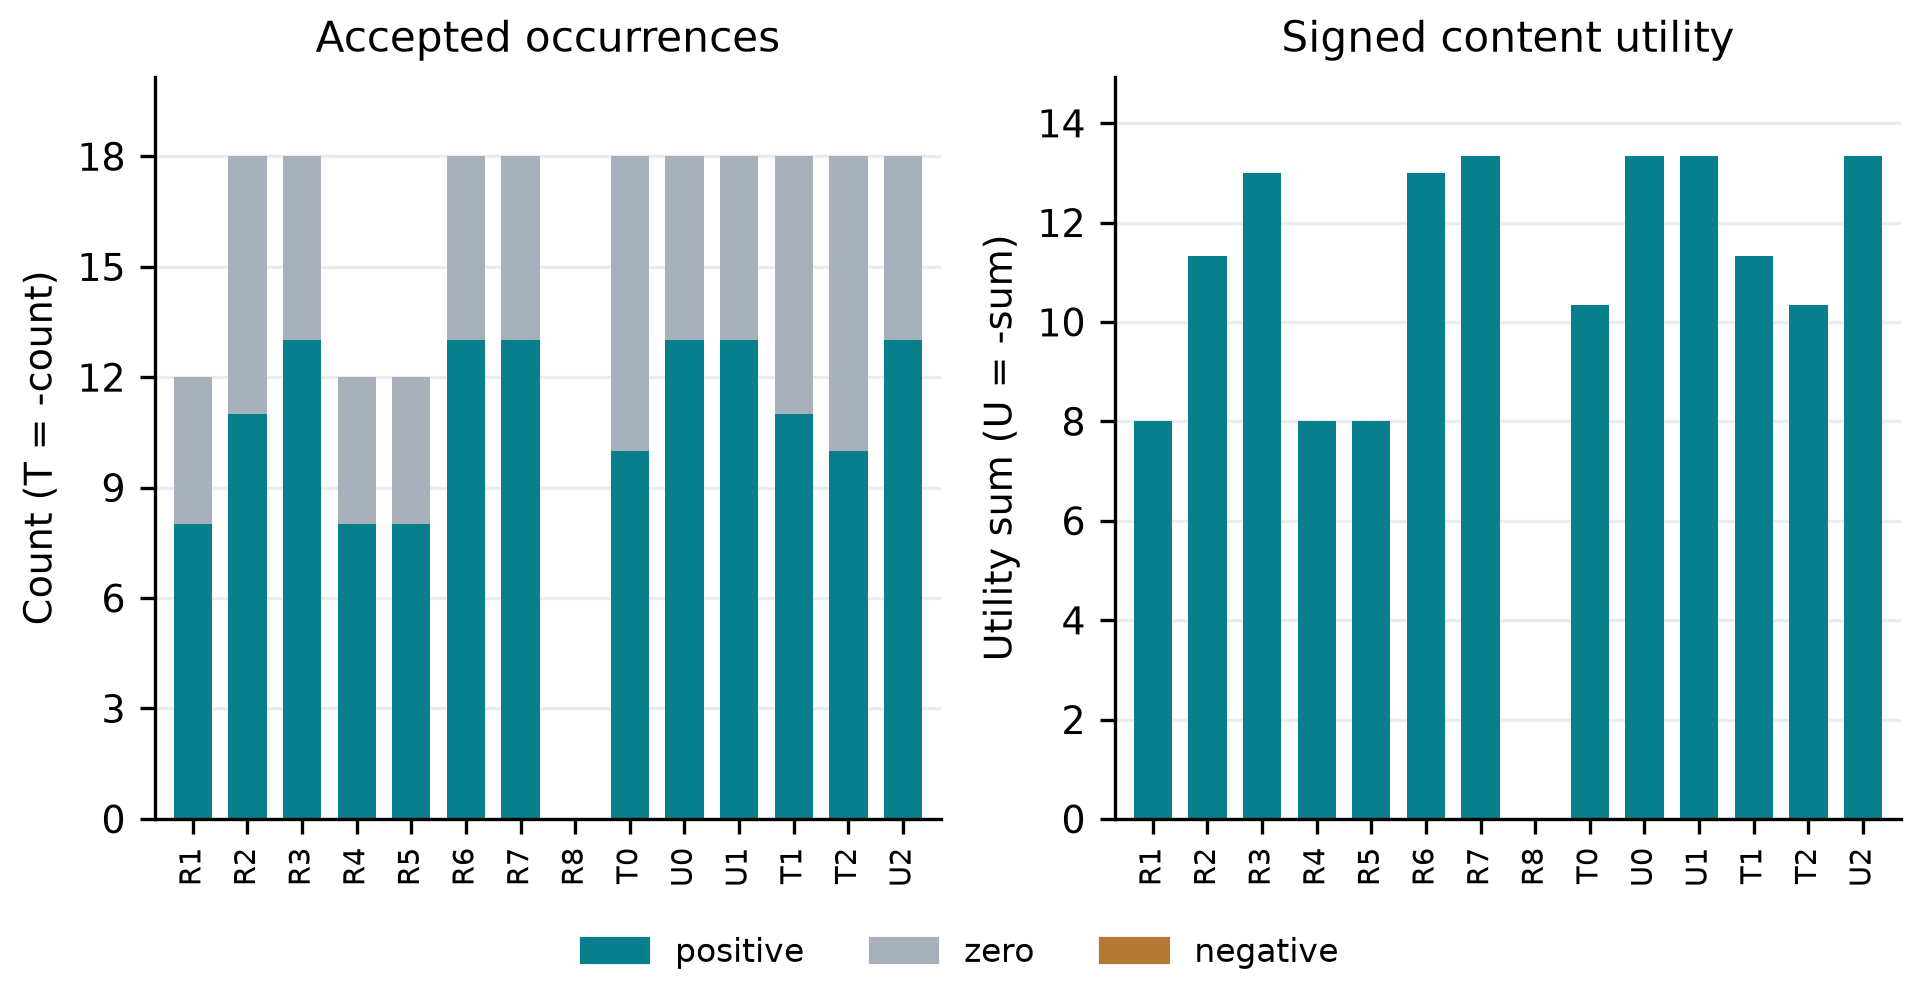
\includegraphics[width=\linewidth]{figures/native-planning-paper-v1/content-contributions.png}
\caption{Every accepted occurrence and its signed fixed-content contribution.
All14 worlds remain in the original order; R8 has zero accepted records, not
a missing observation. No negative contribution appears in these realized
accepted sets. The panel is an opinion instrument, not a truth oracle or a
rerating of rejected and unproduced contents.}
\label{fig:planning-content}
\end{figure}

Execution takes13,014.325s (3h36min54s), with about5min15s to double audit/cost
closure and another66s to the last reader. There are2,019 completed scientist
responses,2,196,668 input and194,184 output tokens;368,423 cached prompt tokens
are a subset of input. Fixed-content measurement uses162 critic POSTs for54
three-position panels, with77,940 input and24,002 output tokens. Designer
authoring records86 POSTs with3,598,980 input/8,820 output tokens; readiness
records200 POSTs with3,843,374 input/9,844 output tokens. Thirteen designer and
fourteen scientist loads have unknown token usage. Categories stay separate;
missing costs are not zero-filled, and no energy or money estimate is inferred.

This closes a functioning feedback-bearing native search, not useful automatic
invention. The prepared selection-fixed evaluator has not been dispatched for
these programs; no unused seed is chosen. More flat evaluation alone would
not distinguish objective support from narrow proposal coverage. A substantive
follow-up must separate action choices and proposal information before making
method-general claims, and independently evaluate whatever fixed systems and
design procedures that question concerns.
\FloatBarrier
